\documentclass{article}
\usepackage{amsmath}
\usepackage{graphicx}
\usepackage{fullpage}


\begin{document}
\title{Preliminary Results}
\author{Shelby Scott}
\date{\today}
\maketitle

\section*{Covariates of Gun Crime}
\begin{table}[htbp] \centering
 \label{SES_Categories}
 \begin{tabular}{|l|l|} \hline
  \textbf{Variable} & \textbf{Description} \\\hline
  Crowding & Percent of occupied housing units with more than one person per room \\\hline
  Poverty & Percent of households living below the federal poverty level \\\hline
  Unemployment & Percent of persons aged 16 years or older in the labor force that are unemployed \\\hline
  Education & Percent of persons aged 25 years or older without a high school diploma \\\hline
  Dependents & Percent of the population under 18 or over 64 years of age \\\hline
  PCI & Per Capita Income \\\hline
  Hardship & A score that incorporates each of the selected socioeconomic indicators \\\hline
 \end{tabular}
 \caption{Descriptions of the variables from the selected socioeconomic indicators in Chicago, 2008-2012 data set.}
\end{table}

\begin{table}[htbp] \centering
\label{AICResults}
 \begin{tabular}{|l|c|} \hline
  \textbf{Subset} & \textbf{AIC Value} \\\hline
  $0~2~3~5$ & $862.73$ \\\hline
  $0~1~3~5$ & $863.68$ \\\hline
  $0~2~3~5~6$ & $863.69$ \\\hline
  $0~1~2~3~5$ & $863.77$ \\\hline
  $0~2~3~4~5$ & $864.42$ \\\hline
 \end{tabular}
\caption{The results of a subset selection procedure with a negative binomial regression and AIC as the diagnostic criteria.}
\end{table}

\begin{table}[htbp] \centering
\label{SubsetParameters}
 \begin{tabular}{|c|l|l|} \hline
  \textbf{Parameter} & \textbf{Description} & \textbf{Value} \\\hline
  $\alpha$ & Dispersion & $0.7095$ \\\hline
  $\beta$ & Regression Coefficients & $[4.1258, 0.0338, 0.1064, -0.0537]$ \\\hline
  $LogL$ & Log Likelihood & $-427.3667$ \\\hline
  $\delta$ & Objective change at convergence & $4.9554 x 10^{-7}$ \\\hline
 \end{tabular}
 \caption{Diagnostics from the Bayesian subset selection algorithm.}
\end{table}

The covariance matrix of $\beta$ is:

\[ CovB = 
\begin{bmatrix}
 106.3414 & 2330.1 & 1643.9 & 3802.9 \\
 2330.1 & 65035 & 43346 & 87248 \\
 1643.9 & 43346 & 31416 & 62748 \\
 3802.9 & 87248 & 62748 & 141640 \\
\end{bmatrix}
\]

\pagebreak
\section*{Number of Disease States}
\begin{figure}[htbp] \centering
 \label{KClusters}
 \includegraphics[scale=1]{figures/Kselection_15.png}
 \caption{The resulting $f(K)$ values for one iteration of the $K$-selection algorithm.}
\end{figure}

\pagebreak
\section*{Infectiousness of Gun Crime}
 \begin{figure} [htbp] \centering
  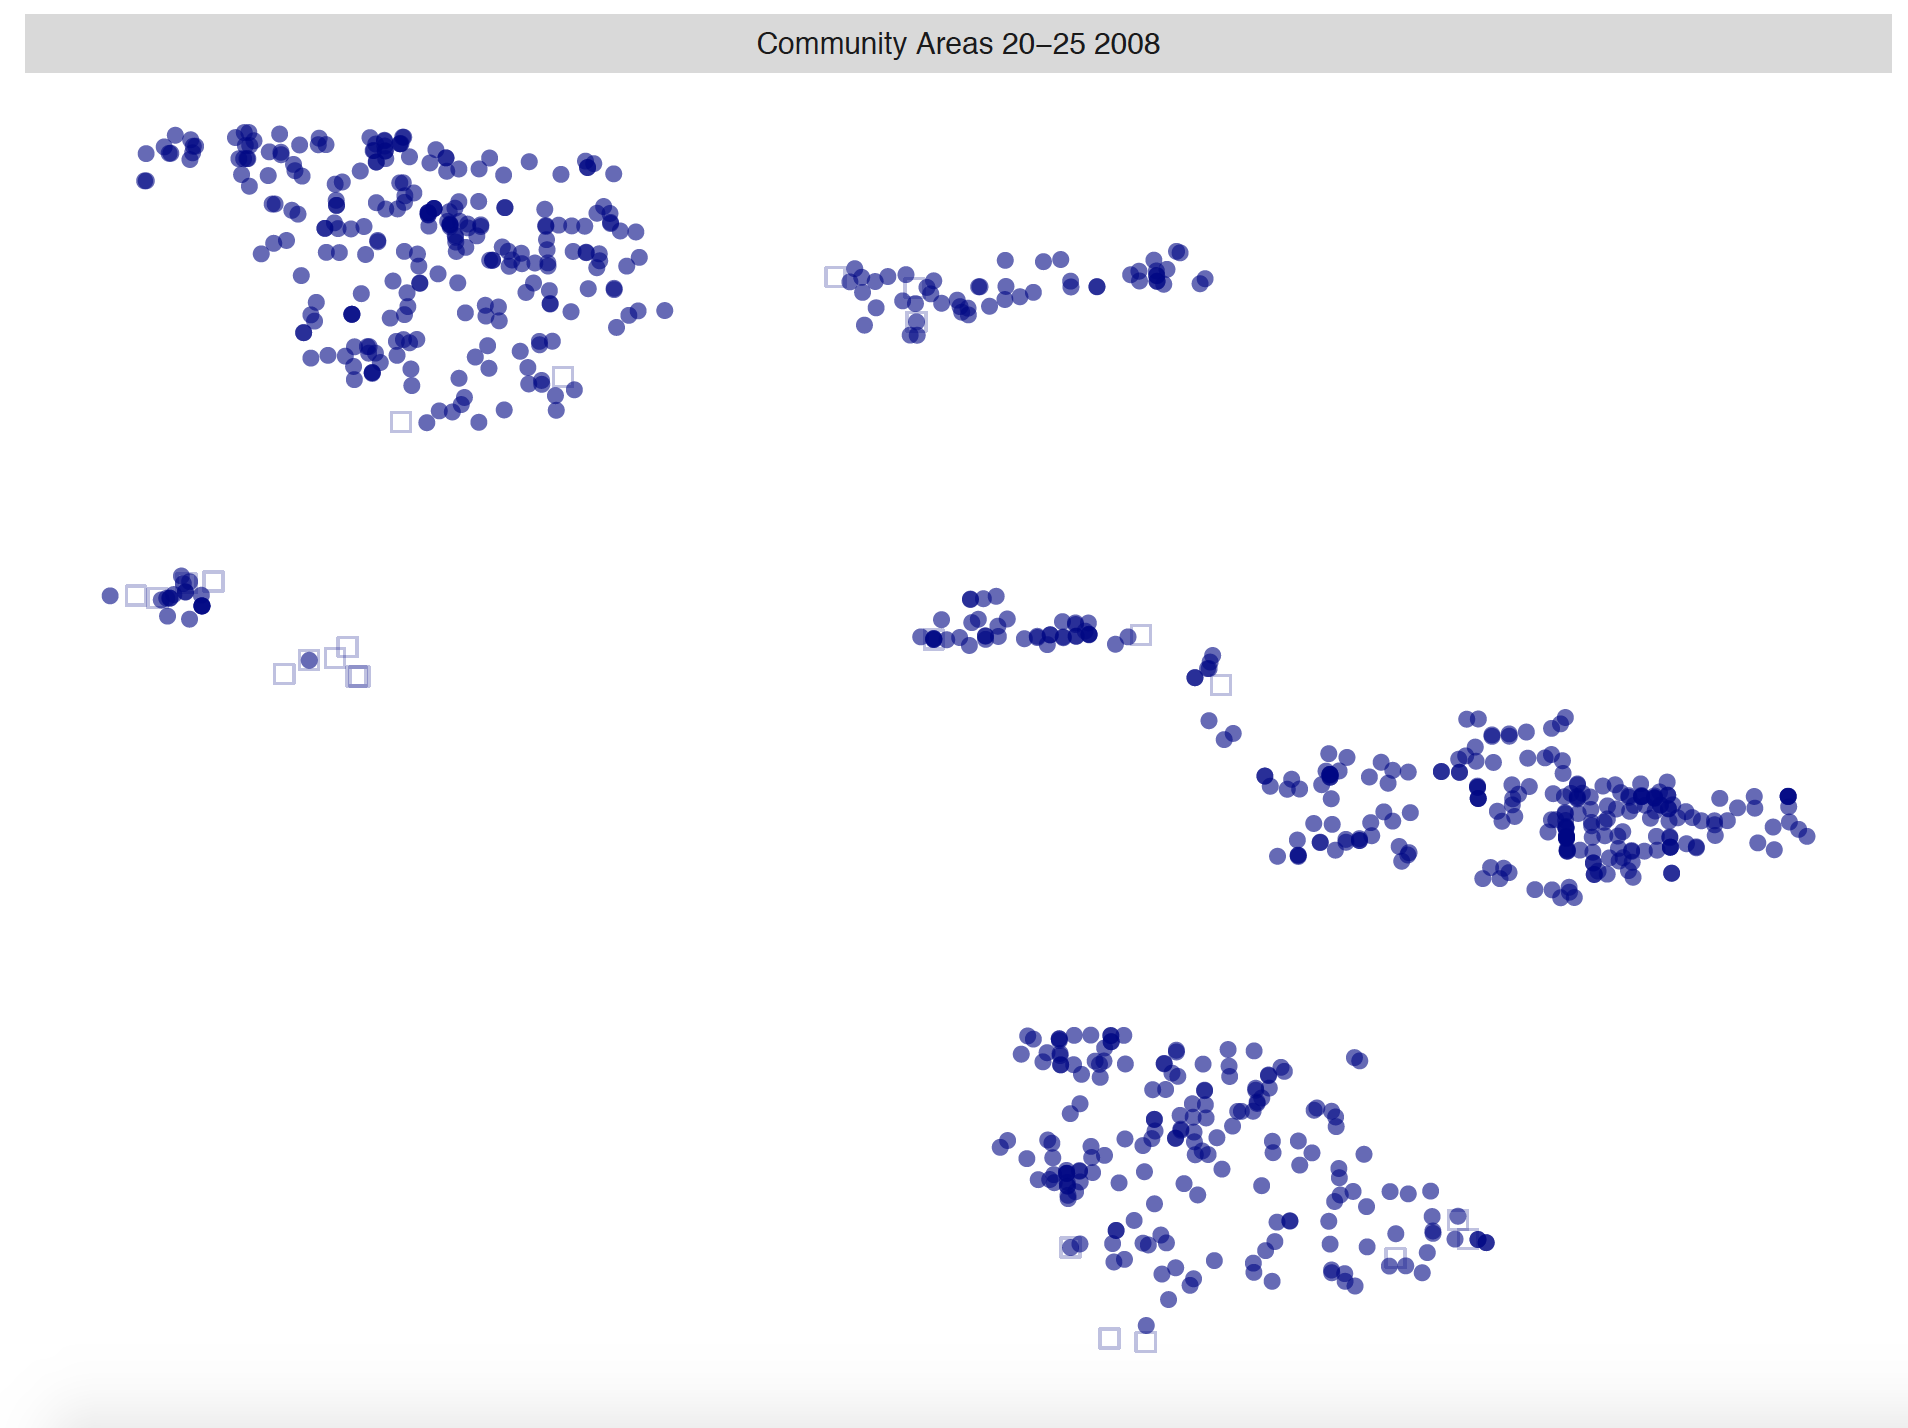
\includegraphics[scale=0.50]{figures/ChicagoCA2025_2008}
  \caption{Map of gun crimes occurring in Chicago community areas 20-25. Open squares are crimes that have not been triggered by past crimes, while filled circles are those which have been triggered.}
  \end{figure}

\end{document}